\section{Solução desenvolvida}
\label{sec:iotGateway}

Esta seção detalha os objetivos e decisões arquiteturais. Foi desenvolvida uma solução de software de \textit{Smart Gateway IoT} que está disponibilizada no Github, capaz de receber dados através de uma rede utilizando o protocolo MQTT	(\ref{mqtt}) de um dispositivo previamente cadastro e armazenar essas informações. Os dados recebidos são analisados para a estrutura que irá definir a execução ou não de um fluxo de notificação através de SMS (\ref{sms}) para um número definido.

\subsection{Tecnologias Utilizadas} 
\begin{itemize}
	\item Node.js \footnote{NodeJS - \url{https://nodejs.org/en/}} v6.x;
	\item TypeScript \footnote{Typescript - \url{http://www.typescriptlang.org/}} v2.3 com transpile para ES6;
	\item TSLint \footnote{TSLint - \url{https://palantir.github.io/tslint/}} v4.x com recomendações gerais padrão;
	\item Jest \footnote{Jest - \url{https://facebook.github.io/jest/}}para teste unitário e cobertura;
	\item AngularJS \footnote{AngularJS - \url{https://angularjs.org/}} v1.6 para o front end da aplicação ;
	\item MongoDB \footnote{MongoDB - \url{https://www.mongodb.com/}} para persistência;
	\item MQTT (\ref{mqtt}) como protocolo de comunicação entre os sensores e o Gateway;
	\item SMS (\ref{sms}) como serviço de mensageria;
	\item ExpressJS \footnote{ExpressJS - \url{http://expressjs.com/}} como framework web Node.js 
\end{itemize}

O Node.js foi escolhido por conta de seu baixo consumo de memória e processamento, além da sua característica de Non-Blocking IO \cite{NodeJSNonBlockingIO}, garantindo que possamos servir mais clientes com menos recursos, objetivo essencial para aplicações que podem ser executadas em um Raspberry Pi por exemplo.

A escolha pelo TypeScript \footnote{Typescript - \url{http://www.typescriptlang.org/}}, linguagem que é um superset do Javascript padrão foi motivada por garantir uma estrutura tipada, de forma que a manutenção do código fosse facilitada e as regras de negócio pudessem estar ligadas a um contrato de objeto.

Já o AngularJS \footnote{AngularJS - \url{https://angularjs.org/}} foi escolhido por ser uma tecnologia que funciona com javascript nativo, sem necessidade de nenhum pós-processador para servir a aplicação aos clientes, permitindo o seu uso diretamente entre os arquivos estáticos do mesmo servidor Node.js que expõe a aplicação. Além disso, contou como um ponto para a escolha, a experiência prévia da equipe no desenvolvimento com esta tecnologia.

\subsubsection{Protocolos de comunicação}
\label{protocolos}

\phantomsection{SMS}\label{sms}, abreviação de \textit{Short Message Service}, é um serviço de troca de mensagens curtas de textos que permite o envio de mensagens para aparelhos celulares, conforme os padrões definidos no GSM (\textit{Global System for Mobile Communications}). Seu uso é bastante popular (cerca de 3,6 bilhões de usuários) \cite{SMS} e ubíquo (presente em praticamente qualquer país) \cite{SMSItu}. Além do que seu uso é fácil e barato, uma vez que o usuário receptor não requer conexão com a Internet para receber a mensagem, bastando possuir sinal com a rede de telefonia.

O \phantomsection{MQTT}\label{mqtt}, abreviação de \textit{Message Queue Telemetry Transport}, é um protocolo de comunicação altamente voltado para IoT. Ele foi arquitetado para ser um sistema de mensageria leve do tipo publisher/subscriber, para rodar em dispositivos limitados, tanto do ponto de vista da quantidade de memória para execução do programa, quanto do ponto de vista da conectividade. Redes lentas ou com alta latência não são problemas para esse protocolo. Geralmente, sensores IoT podem residir em locais extremamente hostis do ponto de vista de infra-estrutura de conexão de dados.

\subsection{Modelo de Dados}
O modelo de dados foi concebido com a intenção de tornar as etapas do processo altamente plugáveis e customizáveis no curto e longo prazo, garantindo as funcionalidades básicas do MVP \footnote{\textit{Minimum Viable Product}, ou Produto Mínimo Viável, é um termo utilizado para caracterizar um produto com as features necessárias para os primeiros clientes \cite{MVP}} executado e a possibilidade de extensibilidade no futuro com retrocompatibilidade. 

Nesta modelagem, a entidade \verb|Dispositivo| identifica um aparelho qualquer que se conecte ao gateway para transmitir informações, o aparelho deve definir um ID de conexão que é cadastrado nesta entidade. Com relação direta a entidade \verb|Dispositivo|, e a entidade \verb|Trigger| modela um gatilho clássico, composto de condição e ação. Nesta perspectiva, a condição é a entidade \verb|Operação| que permite avaliar os valores recebidos e identificar se eles são iguais ou estão no intervalo de valor definidos por esta entidade. A entidade \verb|Evento| por sua vez é a ação, onde é definido o que acontecerá caso a condição seja atendida, por exemplo, o envio de SMS para um destinatário com o determinado texto, ver Figura~\ref{fig:modeloDeDados}.

Além das entidades que servem diretamente a execução do fluxo principal da aplicação, temos 3 entidades de funções secundárias. \verb|Configuracao| é responsável por armazenar os dados utilizados para configurar a aplicação, como a configuração das credenciais para uso do serviço de SMS. As entidades \verb|HistoricoEvento| e \verb|HistoricoMensagem| são responsáveis por armazenar os dados recebidos e os eventos executados.

\begin{figure}[h!]
	\begin{center}
		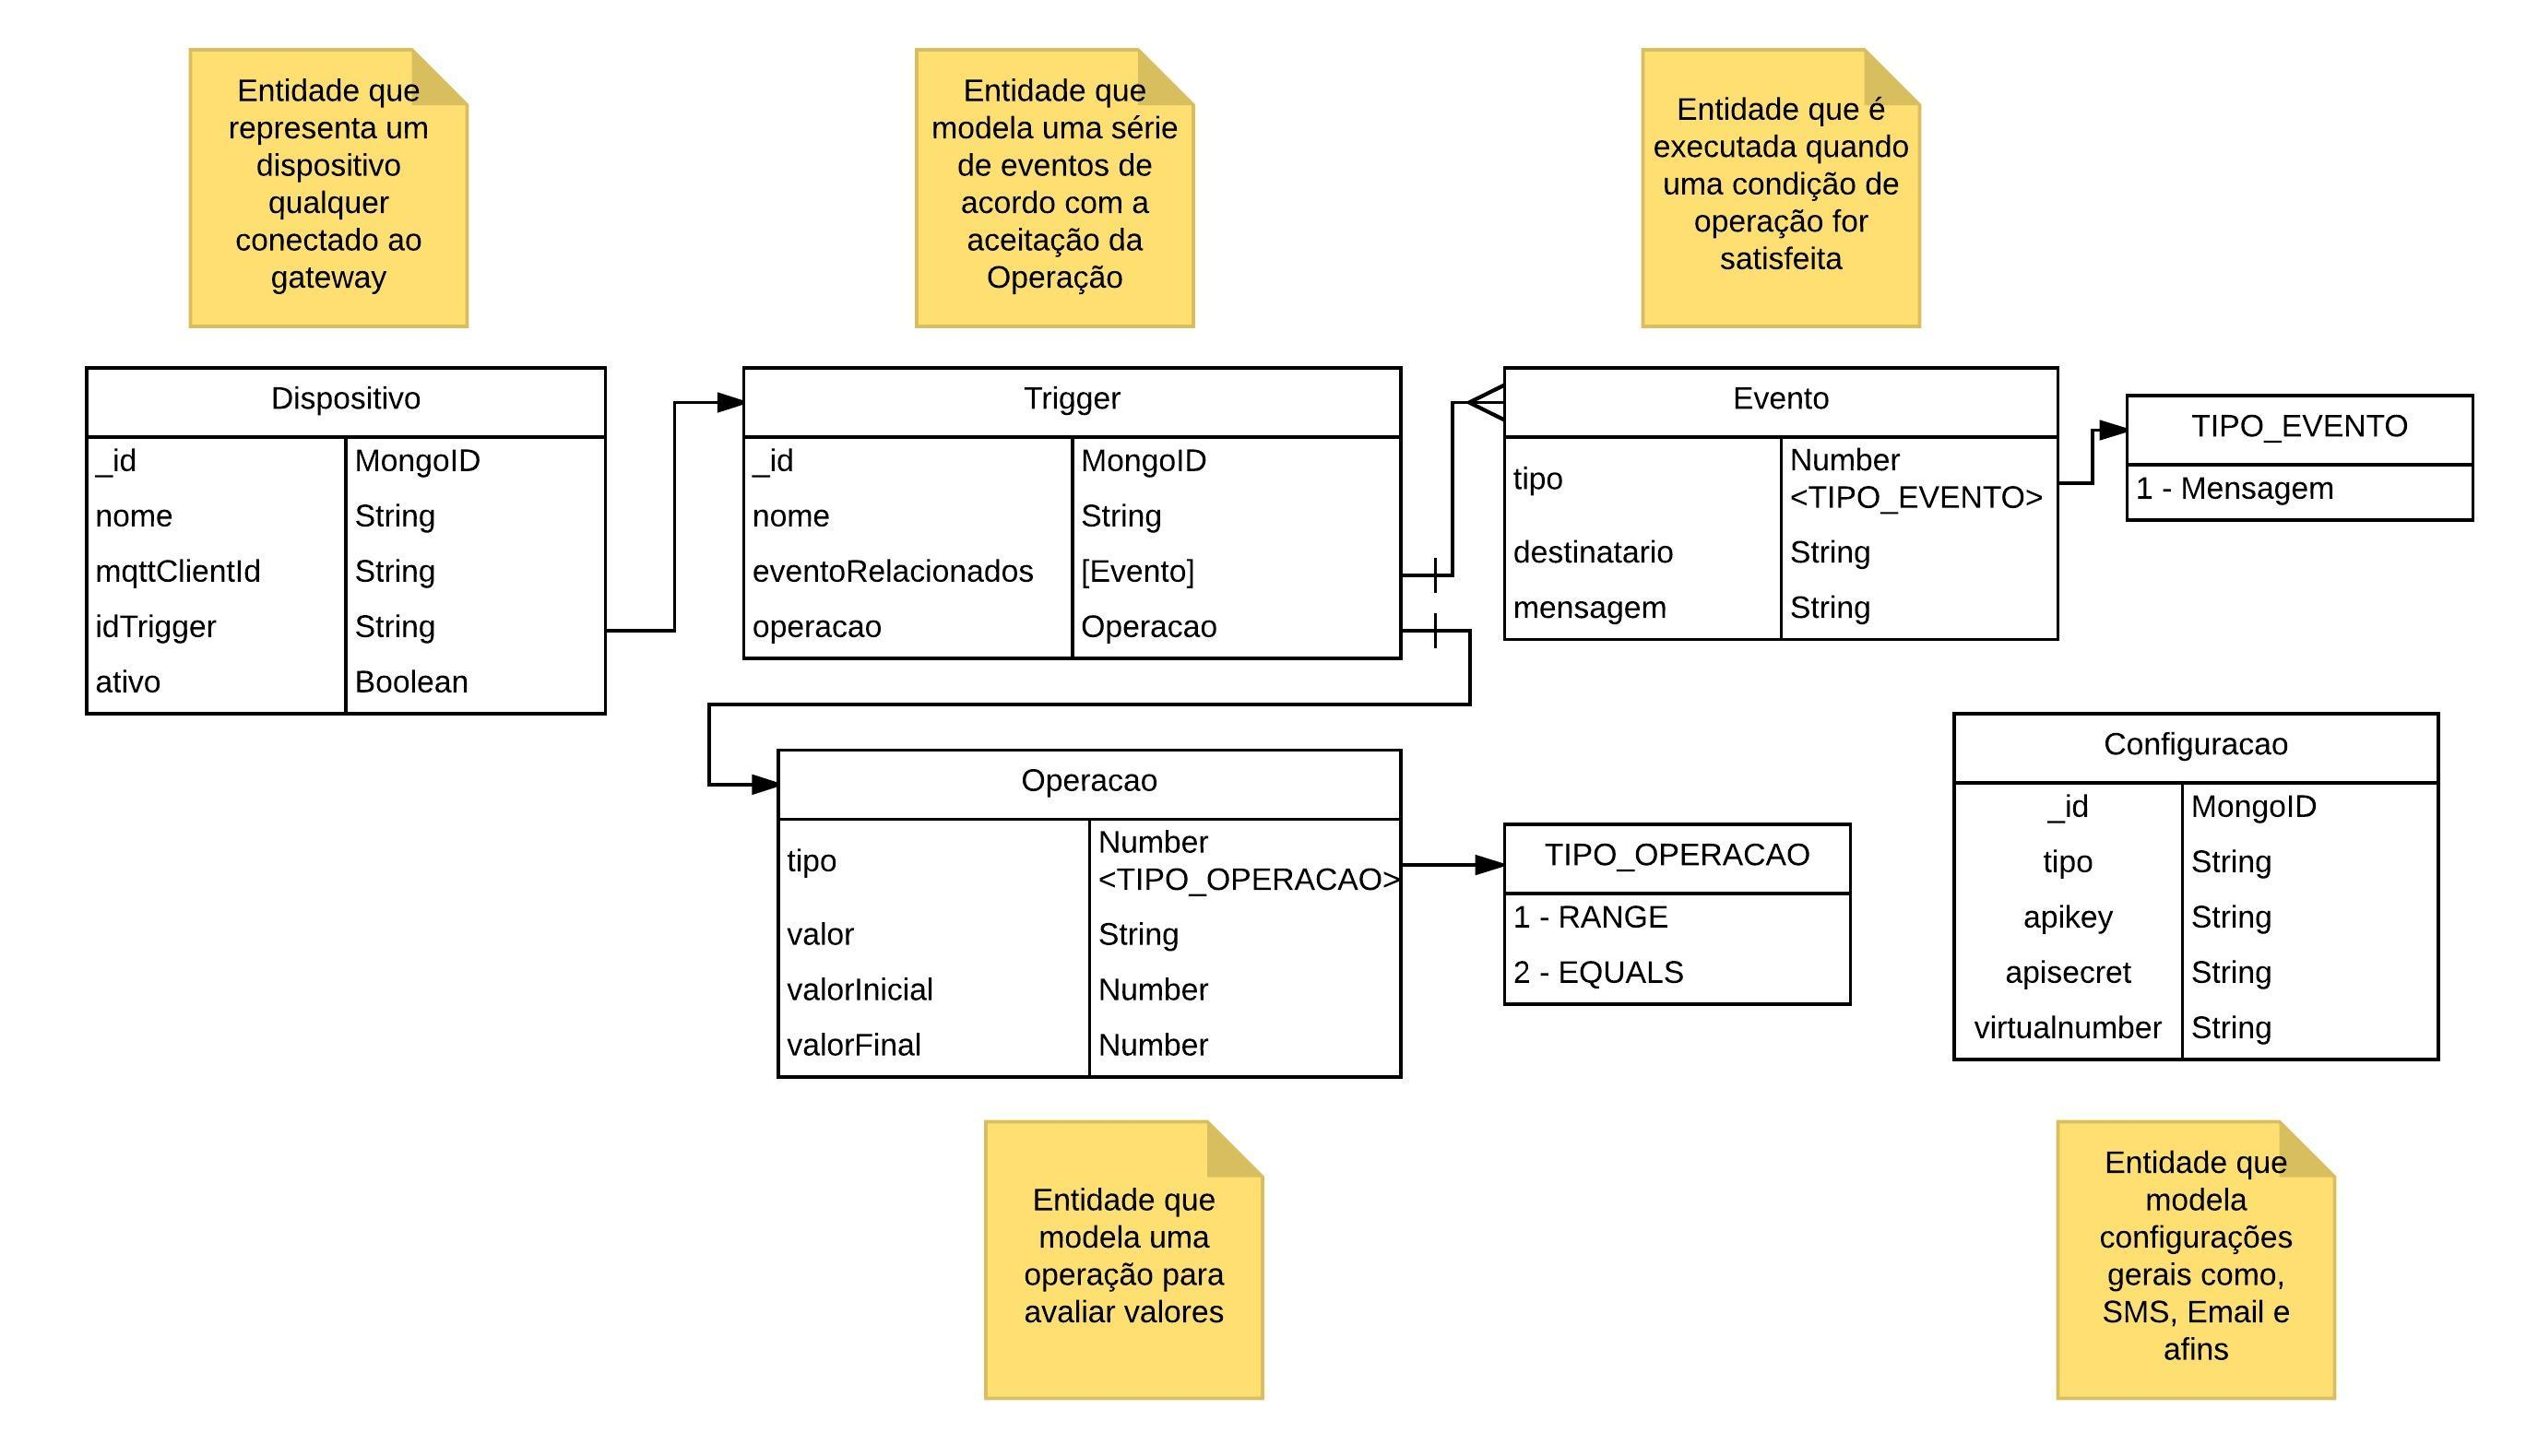
\includegraphics[width=1.085\textwidth]{./img/modelo-de-dados}
		\caption{Representação esquemática da modelagem de dados.}
		\label{fig:modeloDeDados}
	\end{center}
\end{figure}

\begin{figure}[h!]
		\begin{center}
		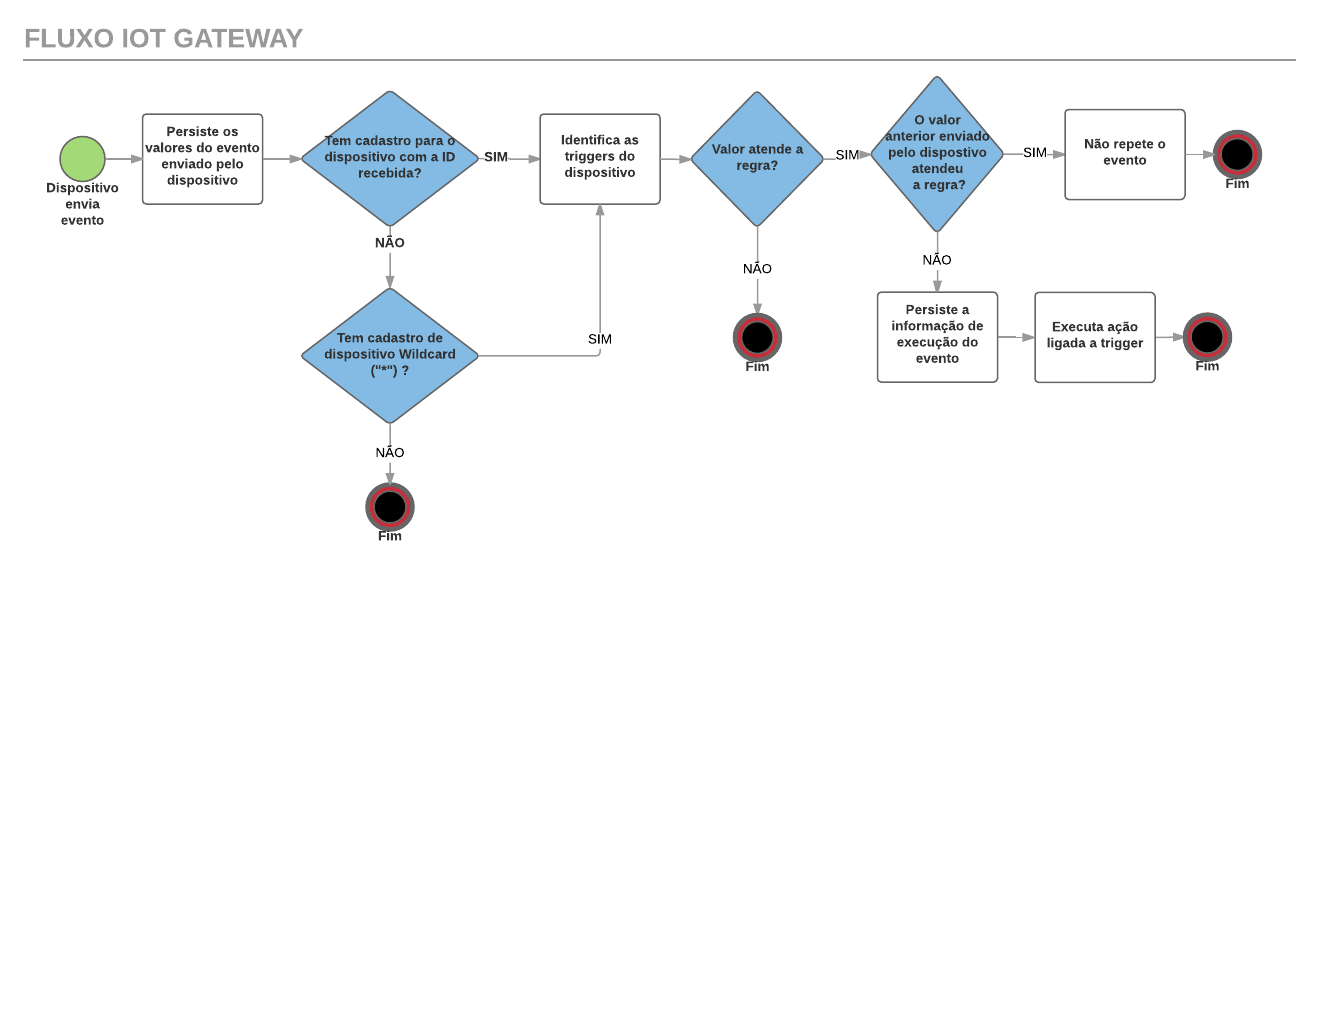
\includegraphics[width=0.9\textwidth]{./img/fluxograma}
		\caption{Representação esquemática do fluxo Gateway IoT.}
		\label{fig:fluxograma}
	\end{center}
\end{figure}

A modelagem desenvolve uma estrutura sequencial que parte da identificação do dispositivo, análise dos gatilhos ligados a este dispositivo, avaliação da operação lógica e liberação para execução do evento, ver Figura~\ref{fig:fluxograma}.  

\subsection{Requisitos funcionais}
\label{reqFuncionais}

Os requisitos funcionais levados em consideração nesse trabalho foram:

\begin{itemize}
	\item Cadastro de dispositivos
	\item Conexão de dispositivos via protocolo MQTT
	\item Visualização e persistência de eventos enviados pelos dispositivos
	\item Envio de mensagens via SMS
	\item Configuração de número(s) de celular como destinatário(s) de SMS enviada
	\item Cadastro de triggers
\end{itemize}

\subsection{Requisitos não funcionais}
\label{reqNaoFuncionais}

Requisitos não funcionais, como os de extensibilidade e de retrocompatibilidade, agregam muito esforço no desenho de um MVP, mas são aspectos que em hipótese alguma podem ser desconsiderados.

Uma vez que a linguagem escolhida (o Typescript) permite o uso conceitos de Orientação à Objetos (tais como abstrações, tipagens, interfaces e herança), a extensibilidade pode ser garantida por meio da inclusão de novos módulos Typescript e pela extensão do modelo de entidades. Ambos os módulos já existentes e os novos coexistiriam sem muitas dificuldades, garantindo assim a retrocompatibilidade.

O componente \verb|EventoApi.ts|~\footnote{https://github.com/RicardoRFaria/IoT-Gateway/blob/master/src/api/EventoApi.ts} é responsável pelo chaveamento entre as implementações de envio de evento. Vejamos abaixo um trecho de código desse componente:

\lstinputlisting[language=JavaScript, caption=EventoApi.ts]{code/EventoApi.ts}

Em relação ao componente acima, caso seja necessário adicionar uma nova forma de envio de evento, basta:

\begin{itemize}
	 \item Injetar a dependência (\verb|import|) (linhas 1 a 4);
	 \item Incluir um novo atributo (linha 11); 
	 \item Instanciar o objeto no construtor (linha 14);
	 \item Alterar o método \verb|executarEvento|, fazendo o devido chaveamento conforme o tipo da implementação (linha 22);
	 \item Criar uma \verb|function| específica para tratar o novo tipo de envio.
\end{itemize}

As configurações específicas da nova forma de envio de eventos poderiam facilmente ser acomodadas na entidade existente de configuração, \verb|Configuracao|, uma vez que a natureza \textit{schemaless} do MongoDB permite esse tipo de cenário.

A compatibilidade com dispositivos cujo hardware possui poucos recursos computacionais, tais como o Raspberry Pi, é o principal requisito não funcional.